\documentclass[uplatex,dvipdfmx,titlepage]{jsarticle}
% \usepackage[top=2.5cm, bottom=2.5cm]{geometry}
\usepackage{amsmath,amssymb,amsthm}
\usepackage{mathtools}
\usepackage{mathrsfs}
\usepackage{graphicx,hyperref}
\usepackage{here}
\usepackage{enumerate}
\usepackage{algorithm}
\usepackage{algpseudocode}
\usepackage{colortbl}
\usepackage{color}
\usepackage{listings}
\usepackage{tikz}

\DeclareMathOperator*{\argmin}{arg\,min}
\DeclareMathOperator*{\argmax}{arg\,max}
\DeclareMathOperator*{\rank}{rank}

\newcommand{\transposed}[1]{#1^\mathsf{T}}

\newtheorem{lemma}{Lemma}
\newtheorem{theorem}{Theorem}
\newtheorem{proposition}{Proposition}
\newtheorem{definition}{Definition}


\title
{
    \begin{Large}
        「数値解析」
    \end{Large}
    \begin{large}
        Aセメスター 月4 \\教員: 松尾 宇泰 先生\\
    \end{large}
    \vspace{15pt}
    \begin{Large}
        期末レポート課題\\
    \end{Large}
    \vspace{20pt}
    \begin{Huge}
      多項式係数補間アルゴリズムの比較
      % Precision comparison of\\
      % polynomial coefficients interpolation
    \end{Huge}
    \vspace{100pt}
}

\author{
  \begin{Large}
    J4-190507 木下裕太
  \end{Large}
}

\begin{document}
  \maketitle

  \section{Preliminary}

  一般に Polynomial interpolation (多項式補間)とは以下のように定式化される問題である.
  \begin{quote}
    INSTANCE:
    \begin{quote}
      \begin{itemize}
        \item 正の整数$n$
        \item 相異なる$n$個の実数$x_1, \ldots , x_n$
        \item $n$個の実数$y_1, \ldots , y_n$\\
      \end{itemize}
    \end{quote}

    QUESTION:
    \begin{quote}
      高々$n-1$次の実係数多項式$f(x)$であって, 次を満たすもの.
      \begin{equation}
        f(x_i) = y_i \quad \forall i \in \{1, \ldots, n\}
      \end{equation}
    \end{quote}
  \end{quote}
  まず次の基本事項を確認しておく.

  \begin{theorem}
    Polynomial interpolation はちょうど一つの解をもつ.
  \end{theorem}

  \begin{proof}2つのパートに分けて示す.
    \begin{itemize}
      \item Existence\\
      次のように定まる多項式は(1)を満たしている.
      \begin{eqnarray}
        f(x) = \sum_{i=1}^n y_i\prod_{j\neq i} \cfrac{x-x_j}{x_i-x_j}
      \end{eqnarray}

      \item Uniqueness\\
      高々$n-1$次の実係数多項式$f(x),g(x)$が共に(1)を満たすとする.
      このとき$(f-g)(x)$も高々$n-1$次であり
      \begin{eqnarray*}
        (f-g)(x_i) = 0 \quad \forall i \in \{1, \ldots, n\}
      \end{eqnarray*}
      を満たすので, 因数定理より
      \begin{eqnarray*}
        f-g=0\\
        \therefore \quad f=g
      \end{eqnarray*}
    \end{itemize}
  \end{proof}

  本レポートは QUESTION を次に代えた問題(これをCoefficients interpolationと呼ぶことにする)を対象とする.
  \begin{quote}
    QUESTION:
    \begin{quote}
      $n$個の実数$a_0, \ldots, a_{n-1}$であって, 次を満たすもの.
      \begin{equation}
        \sum_{k=0}^{n-1} a_k x_i^k = y_i \quad \forall i \in \{1, \ldots, n\}
      \end{equation}
    \end{quote}
  \end{quote}
  初めの問題との違いは, 求める多項式を具体的に係数列として要求する点のみである.
  したがって前者を解くアルゴリズムから直ちに本問題の解法も得ることができる.
  Section 2 では実際にいくつかのアルゴリズムを検討する.

  ここで注目したいのが, 実用上それらの手法による補間はどこまで正確な値を得られるのかということである.
  例えば, 未知の関数をべき級数に展開した際の係数列から必要な情報を取り出したい場面などにおいて, このような復元精度の見積もりは重要な話題であると考えられる.
  Section 3 ではインスタンスのサイズや標本点の取り方を変化させたときに誤差がどのような振る舞うかを, それぞれの補間アルゴリズムについて測定し比較する.

  \section{Algorithms}
  本章では Coefficients interpolation を解くアルゴリズムをいくつか紹介する.
  ここで取り上げた手法はいずれも次章で測定の対象とする.

  \subsection{Lagrange interpolation}
  式(2)による補間はLagrange interpolation (ラグランジュ補間)と呼ばれる.
  これを展開して式(3)の形にするというのは自然なアイデアである.

  まず式(2)を項別に計算してそれらの和をとるナイーブな方法を考える。
  多項式の積を愚直に計算する場合, 全体の時間計算量は $\Theta(n^3)$ となり, 畳み込みにFFTを用いると $\Theta(n^2 \log n)$ である.

  さらに式(2)は
  \begin{eqnarray}
    p(x) = \prod_{i = 1}^n (x-x_i)
  \end{eqnarray}
  を用いて
  \begin{eqnarray}
    f(x) &=& \sum_{i=1}^n y_i\prod_{j\neq i} \cfrac{x-x_j}{x_i-x_j} \nonumber\\
    &=& \displaystyle\sum_{i=1}^n y_i \prod_{j\neq i}(x_i-x_j)^{-1} \cfrac{p(x)}{x-x_i}
  \end{eqnarray}
  と表せる.
  式(4)の右辺を$O(n^2)$で前計算しておけば, 式(5)の各項は $\Theta(n)$ で求めることができ, 全体として $\Theta(n^2)$ に改善できる.

  \subsection{Vandermonde matrix}
  次に Vandermonde 行列を用いた方法を考える.
  Coefficients interpolation は次の連立一次方程式として言い換えることができる.
  \begin{eqnarray}
    V(x)a = y
  \end{eqnarray}
  ただし $V(x)$はVandermonde 行列
  \begin{eqnarray}
    V(x)
    = \left(\begin{matrix}
      1 & x_1 & \cdots & x_1^{n-1}\\
      \vdots & \vdots & \ddots & \vdots\\
      1 & x_n & \cdots & x_n^{n-1}\\
    \end{matrix}\right)
  \end{eqnarray}
  である.

  方程式(7)を特別な性質を用いずに解くと計算量は$\Theta(n^3)$となる.
  ここで次の事実を活かすことができる.

  \begin{theorem}
    下三角行列$L(x)$を
    \begin{eqnarray}
      L(x) &=& \left(\begin{matrix}
        1 &\\
        1 & x_2-x_1\\
        1 & x_3-x_1 & (x_3-x_1)(x_3-x_2)\\
        \vdots & \vdots & \vdots & \ddots \\
        1 & x_n-x_1 & (x_n-x_1)(x_n-x_2) & \cdots & \displaystyle\prod_{i=1}^{n-1}(x_n-x_i)
      \end{matrix}\right)
    \end{eqnarray}
    で, 上三角行列$R(x)$を
    \begin{eqnarray}
      R(x) &=& \left(\sum_{d\in D_{r, c-r}} \prod_{i=1}^{r} x_i^{d_i}\right)_{r\le c}
      \quad \text{with} \quad D_{n, m} = \{d \in \mathbb{Z}_{\ge 0}^n \mid \sum_{i=1}^n d_i = m\}
    \end{eqnarray}
    で定める.
    このとき
    \begin{eqnarray}
      V(x) = L(x) U(x)
    \end{eqnarray}
    が成り立つ.
  \end{theorem}

  \begin{proof}
    $n$についての帰納法から示すことができるが, やや冗長なため割愛.
  \end{proof}

  $L(x), R(x)$ともに対角成分は$0$でないため, $V(x)$は正則行列であることが確認できる.\footnote{Proposition 1 の別証となっている.}
  重要な事実として, シンプルな動的計画法によって(10), (11)の全ての成分を$\Theta(n^2)$時間で計算することができる.\footnote{詳細は実装を参照されたい.}
  Backward substitution は$\Theta(n^2)$で動作するので, (7)を時間計算量$\Theta(n^2)$で解くことができた.

  なおこのアルゴリズムの注意点として, 一般にVandermonde 行列は条件数の大きい変換として知られており\cite{1}, 他の手法と比べて特に数値解が安定しない懸念がある.

  \subsection{Fast interpolation}
  最後に, Polynomial interpolationを (現時点で) 最も高速に解くアルゴリズム\cite{2}として知られているものを取り上げる.
  時間計算量は $O(n (\log n)^2)$である.

  その前に, 本アルゴリズムの中で部分問題として現れる Multipoint evaluation (多点評価)について述べておく. その内容は次の通りである.
  \newpage
  \begin{quote}
    INSTANCE:
    \begin{quote}
      \begin{itemize}
        \item 正の整数$n$
        \item 相異なる$n$個の実数$x_1, \ldots , x_n$
        \item $n$個の実数$a_0, \ldots , a_{n-1}$\\
      \end{itemize}
    \end{quote}

    QUESTION:
    \begin{quote}
      $n$個の実数$y_1, \ldots, y_n$であって, 次を満たすもの.
      \begin{equation*}
        \sum_{k=0}^{n-1} a_k x_i^k = y_i \quad \forall i \in \{1, \ldots, n\}
      \end{equation*}
    \end{quote}
  \end{quote}
  見ての通り, Multipoint evaluation と Coefficients interpolation は互いに逆問題の関係にある.
  Multipoint evaluation についても, 現在達成されている最良の計算量は$O(n(\log n)^2)$であり,
  以下で紹介するアルゴリズムはこれをサブルーチンとして用いる.

  さて本題に戻る. 鍵となるのは Subproduct tree と呼ばれるデータ構造である.
  これは Labeled binary tree の構造をなし, 各内部ノードがもつ値はその子ノードのもつ値の積に等しいという性質をもつ.
  アルゴリズムの大まかな流れは次のようになる.\footnote{詳細は実装を参照されたい.}

  \begin{enumerate}
    \item $n$個の葉にそれぞれ多項式$x-x_i$をもたせた Subproduct tree $T$を構築する. $T$の各ノードは多項式を係数ベクトルとして保持する.
    \item $T$をボトムアップに見ていき, $q(x) = \displaystyle\sum_{i=1}^n\prod_{j\neq i}(x-x_j)$ を計算する.
    \item サブルーチン\footnote{実はこれもSubproduct tree techniqueを用いている.}を用いて $q(x)$ を $x_1, \ldots, x_n$の各点で評価する.
    \item 3の結果と$y_1, \ldots, y_n$を用いて再び$T$をボトムアップに見ていくことで, (2) の右辺が計算できる.
  \end{enumerate}

  この手法の懸念としては, サブルーチンの中で多項式除算を繰り返し行うことで誤差が大きくなってしまうことが考えられる.

  \section{Benchmarks}
  \subsection{Method}
  以下の実行環境で計算および測定を行った.
  \begin{itemize}
    \item CPU: Intel Core i5
    \item Memory: 8GB
    \item OS: Windows 10
    \item Language: C++ (GCC 10.2.0)
  \end{itemize}

  数値型として64bitの浮動小数点数を用いた.
  その都合上, 係数の絶対値が$1$未満かつ次数が$25$以下であるような多項式が解となるようにテストケースを作成した.
  また標本点についても絶対値が$1$未満となるようにした.
  これらのパラメータは全て一様分布から無作為に抽出して得たものである.

  今回のベンチマークでは, 得られた係数ベクトルを$\hat{a}$, 真値を$a$とするとき,
  \begin{eqnarray}
    \delta_a(\hat{a}) = \cfrac{1}{n}\sum_{i=0}^{n-1}\cfrac{|\hat{a}_i - a_i|}{\max\{1, |a_i|\}}
  \end{eqnarray}
  を評価値とした.
  各$n$ごとに, 先述した方法で作った$50$ 個程度のインスタンスに対してプログラムを走らせ, (11) の値の平均をとったものを片対数グラフにプロットした.
  本測定では低次の多項式のみを扱うため, アルゴリズムによって実行時間に大きな差はないと考え, 時間計測は行わなかった.

  \subsection{Results}
  \begin{figure}[ht]
    \centering
    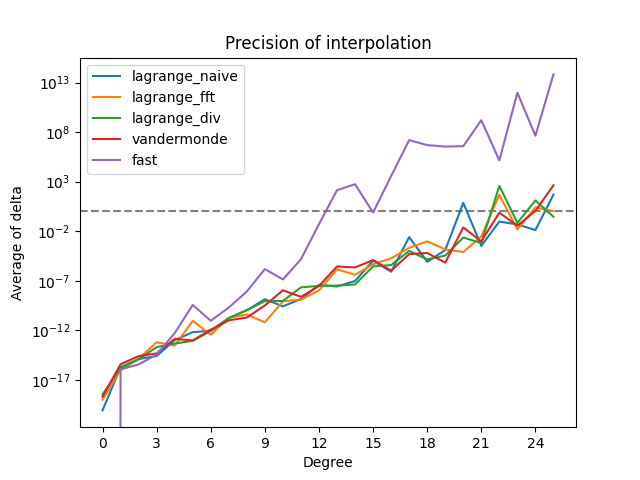
\includegraphics{../test/fig.png}
    \caption{補間精度の比較}
    \label{1}
  \end{figure}

  図\ref{1}から明らかなように, Fast interpolationで得られる数値解は極めて不安定であり, 高々$15$次程度の多項式であっても復元の精度が非常に悪くなりうることがわかる.
  これに関しては前章で述べたように, 多項式除算を含め FFT の実行回数が他に比べて多くなることが原因だと考えられる.
  また他の手法の間にあまり差はなかったが, いずれも相対誤差$10^{-2}$が保証されるのはおよそ次数が$20$以下の場合に限られる.

  \appendix
  \section{Implementation}
  下記のリンクからソースコードにアクセスできる.
  \begin{quote}
    \url{https://github.com/jellc/numerical_analysis}
  \end{quote}

  \begin{thebibliography}{5}
    \bibitem{1} Gautschi, W., \& Inglese, G. (1987). Lower bounds for the condition number of Vandermonde matrices. Numerische Mathematik, 52(3), 241-250.
    \bibitem{2} Aho, A. V., \& Hopcroft, J. E. (1974). The design and analysis of computer algorithms. Pearson Education India.
  \end{thebibliography}
\end{document}
